\documentclass[a4paper,12pt]{article} % тип документа
\usepackage[margin=1in]{geometry} % Поля

%  Русский язык
\usepackage[warn]{mathtext}
\usepackage[T2A]{fontenc}			% кодировка
\usepackage[utf8]{inputenc}			% кодировка исходного текста
\usepackage[english,russian]{babel}	% локализация и переносы
% Математика
\usepackage{amsmath,amsfonts,amssymb,amsthm,mathtools} 
\usepackage{wasysym}
%%%
\usepackage{graphicx}

\usepackage{tabularx}

\usepackage{gensymb} % знак градуса
\usepackage{enumitem} % изменить список enumerate
\usepackage{placeins} % \FloatBarrier

\renewcommand{\thesection}{\Roman{section}} 
\renewcommand{\thesubsection}{\roman{subsection}}


\begin{document}

\newcolumntype{Y}{>{\centering\arraybackslash}X} %new tabularx


%титул
\hrule 	
\medskip
\begin{raggedright}
{\large \textbf{Отчёт по работе 4.8}}
\\
\medskip
{\Large Резонанс напряжений} 
\\
\medskip
{\large Карташов Констанин Б04-005}
\medskip
\hrule
\medskip
\end{raggedright}


\section{Анотация}

\paragraph{Цель работы:} 
Исследование последовательной цепи постоянного тока, наблюдение резонанса напряжений.

\paragraph{Оборудование:}
\begin{itemize}
\renewcommand{\labelitemi}{$\triangleright$}
\itemsep0em
\item Регулировочный автотрансформатор
\item Катушка индуктивности с выдвижным сердечником	
\item Магазин ёмкостей
\item Резистор
\item Амперметр
\item Три вольтметра
\item Ваттметр
\item Осциллограф
\item Универсальный мост
\end{itemize}


\medskip\hrule\medskip

\section{Теоретическая часть}


\begin{figure}[h]
\begin{center}
\begin{minipage}[h]{0.49\textwidth}
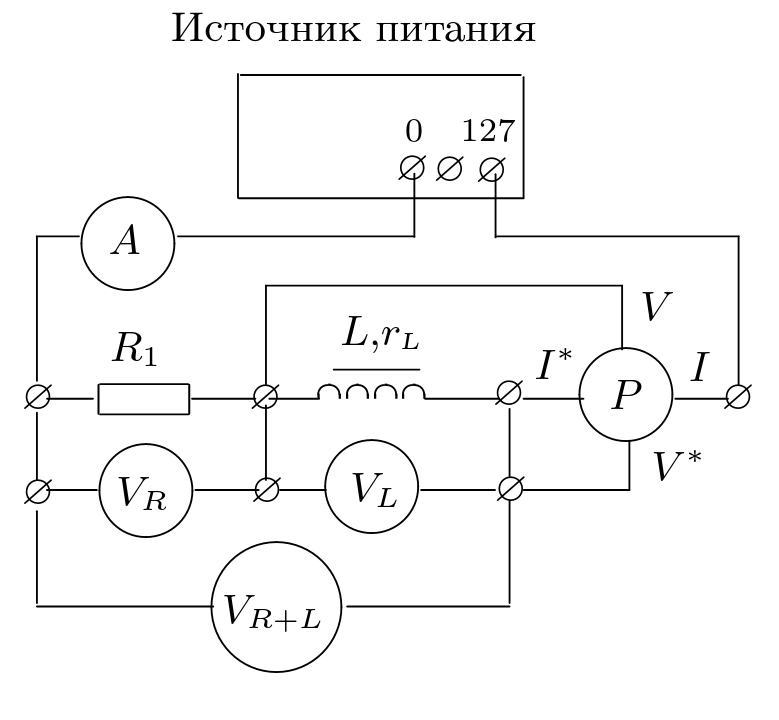
\includegraphics[width=\textwidth]{setup1.png}
\caption{Схема установки для изучения закона Ома в цепи переменного тока}
\label{setup1}
\hfill
\end{minipage}
\begin{minipage}[h]{0.49\textwidth}
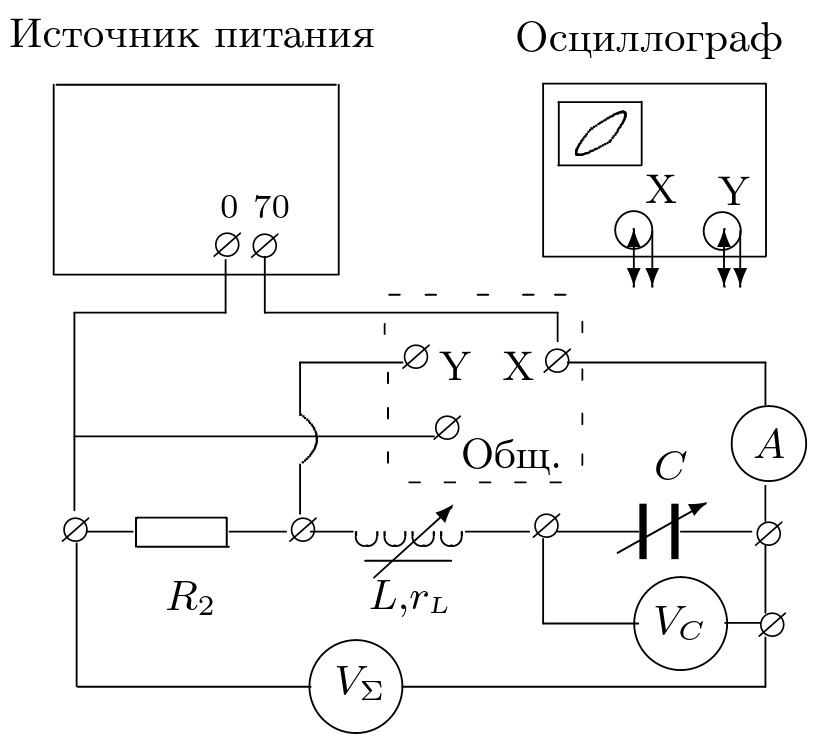
\includegraphics[width=\textwidth]{setup2.png}
\caption{Схема тока для наблюдения резонанса напряжений}
\label{setup2}
\hfill
\end{minipage}
\end{center}
\end{figure}

\paragraph{} Для изучения закона Ома в цепи переменного тока используется установка на рисунке \ref{setup1}. Три вольтметра позволяют нам использовать подробно исследовать напряжения на резисторе и катушке. Для этих напряжений справедливы комплексные соотношения:

\begin{equation}
\hat{U}_R = \hat{I} R, \;\;\; \hat{U}_L = \hat{I} (r_L + i \Omega L), \;\;\; \hat{U}_{R+L} = \hat{I} (R + r_L + i\Omega L).
\label{1}
\end{equation}

Переходя к амплитудам и фазам получаем:

\begin{equation}
U_R = IR, \;\;\; \tg{\psi_1} = 0;  \label{2}
\end{equation}
\begin{equation}
U_L = I \sqrt{r_L^2 + (\Omega L)^2}, \;\;\; 	\tg{\psi_2} = \frac{\Omega L}{r_L};  \label{3}
\end{equation}
\begin{equation}
U_{R+L} = I \sqrt{(R + r_L)^2 + (\Omega L)^2}, \;\;\; 	\tg{\psi_3} = \frac{\Omega L}{R + r_L}.  \label{3}
\end{equation}

Из этих выражений можно получить значение средней мощности выделяемой на катушке. Проинтегрировав $P = I(t) \cdot U(t)$ получаем выражение:

\begin{equation}
\overline{P_L} = U_L \cdot I \cos \psi = I^2 \cdot r. \label{5}
\end{equation}

\paragraph{} Для изучения резонанса используется установке на рисунке \ref{setup2}. В резонансном случае частота вынужденных колебаний совпадает с частотой свободных колебаний контура. В таком контуре совпадают реактивные сопротивления продуктивности и ёмкости:

\begin{equation}
\frac{1}{\omega_0 C} = \omega_0 L. \label{6}
\end{equation}

Добротность такого контура вычисляется по формуле:

\begin{equation}
Q = \frac{\omega_0 L}{R_\Sigma} = \frac{1}{\omega_0 C R_\Sigma}, \;\;\; R_\Sigma = R + r_L. \label{7}
\end{equation}

И в том числе:
\begin{equation}
U_{\Sigma, \; \text{рез}} = I_\text{рез} R_\Sigma, \;\;\; U_{C, \; \text{рез}} = \frac{I_\text{рез}}{\Omega C}. \label{9}
\end{equation}

\begin{equation}
Q = \frac{U_{C, \; \text{рез}}}{U_{\Sigma, \; \text{рез}}}. \label{10}
\end{equation}



\medskip\hrule\medskip

\section{Экспериментальная часть}

\subsection{Снятие зависимости напряжений и тока от положения сердечника катушки}

\paragraph{} Меняя положение сердечника катушки $x$, будем снимать при помощи амперметра значения тока $I$, при помощи вольтметра -- напряжения на резисторе $U_R$, напряжения на катушке $U_L$, суммарное напряжения $U_{L+R}$, и при помощи ваттметра -- мощность выделяемую на цепи $P$. Данные занесём в таблицу \ref{tab:1}.

\begin{table}[h]
\begin{center}
\centering
\begin{tabular}{|l|l|l|l|l|l|}
\hline
\multicolumn{1}{|c|}{$x$, мм} & \multicolumn{1}{c|}{$I$, А} & \multicolumn{1}{c|}{$U_R$, В} & \multicolumn{1}{c|}{$U_{R+L}$, В} & \multicolumn{1}{c|}{$U_L$, В} & \multicolumn{1}{c|}{$P$, Вт} \\ \hline
5 & 1.05 & 45 & 125 & 106 & 24.5 \\ \hline
7 & 1.20 & 52 & 124 & 101 & 23.5 \\ \hline
9 & 1.35 & 57 & 123 & 97 & 22.5 \\ \hline
11 & 1.40 & 61 & 121 & 93 & 21.0 \\ \hline
13 & 1.45 & 63 & 120 & 90 & 20.5 \\ \hline
15 & 1.55 & 66 & 119 & 87 & 20.0 \\ \hline
17 & 1.6 & 69 & 119 & 84 & 19.5 \\ \hline
19 & 1.65 & 71 & 118 & 81 & 19.0 \\ \hline
21 & 1.65 & 73 & 117 & 79 & 18.5 \\ \hline
23 & 1.70 & 74 & 116 & 77 & 18.5 \\ \hline
25 & 1.75 & 75 & 116 & 75 & 18.5 \\ \hline
27 & 1.75 & 77 & 116 & 73 & 18.5 \\ \hline
29 & 1.8 & 78 & 115 & 72 & 18.0 \\ \hline
31 & 1.8 & 79 & 115 & 70 & 18.0 \\ \hline
33 & 1.85 & 80 & 115 & 69 & 18.0 \\ \hline
35 & 1.85 & 81 & 115 & 68 & 18.0 \\ \hline
37 & 1.85 & 82 & 115 & 67 & 17.5 \\ \hline
39 & 1.85 & 82 & 114 & 66 & 17.5 \\ \hline
41 & 1.95 & 82 & 114 & 65 & 17.5 \\ \hline
\end{tabular}
\caption{Напряжения, ток, и мощность при различных положения сердечника}
\label{tab:1}
\end{center}
\end{table}

\paragraph{} По данным из таблицы \ref{tab:1} найдём значения для $r_L$ и $L$ по формулам (\ref{5}) и (\ref{3}). Полученные данные занесём в таблицу \ref{tab:2} и простоим график зависимости $r_L(x)$ и $L_(x)$ (рис. \ref{fig:1}).

\begin{table}[h]
\begin{center}
\begin{tabular}{|c||c|c|c|c|c|c|c|c|c|c|}
\hline 
$x$, мм & 5 & 7 & 9 & 11 & 13 & 15 & 17 & 19 & 21 & 23 \\\hline
$r_L$, Ом & 22.2 & 16.3 & 12.3 & 10.7 & 9.8 & 8.3 & 7.6 & 7.0 & 6.8 & 6.4 \\\hline
$L$, Гн & 0.31 & 0.26 & 0.23 & 0.21 & 0.20 & 0.18 & 0.17 & 0.15 & 0.15 & 0.14 \\\hline
\hline
$x$, мм & 25 & 27 & 29 & 31 & 33 & 35 & 37 & 39 & 41 & -- \\\hline
$r_L$, Ом & 6.0 & 6.0 & 5.6 & 5.6 & 5.3 & 5.3 & 5.1 & 5.1 & 4.6 & -- \\\hline
$L$, Гн & 0.14 & 0.13 & 0.13 & 0.12 & 0.12 & 0.12 & 0.11 & 0.11 & 0.11 & -- \\\hline


\end{tabular} 
\caption{Зависимость индуктивности и активного сопротивления катушки от положения сердечника}
\label{tab:2}
\end{center}
\end{table}

\begin{figure}[h]
\begin{center}
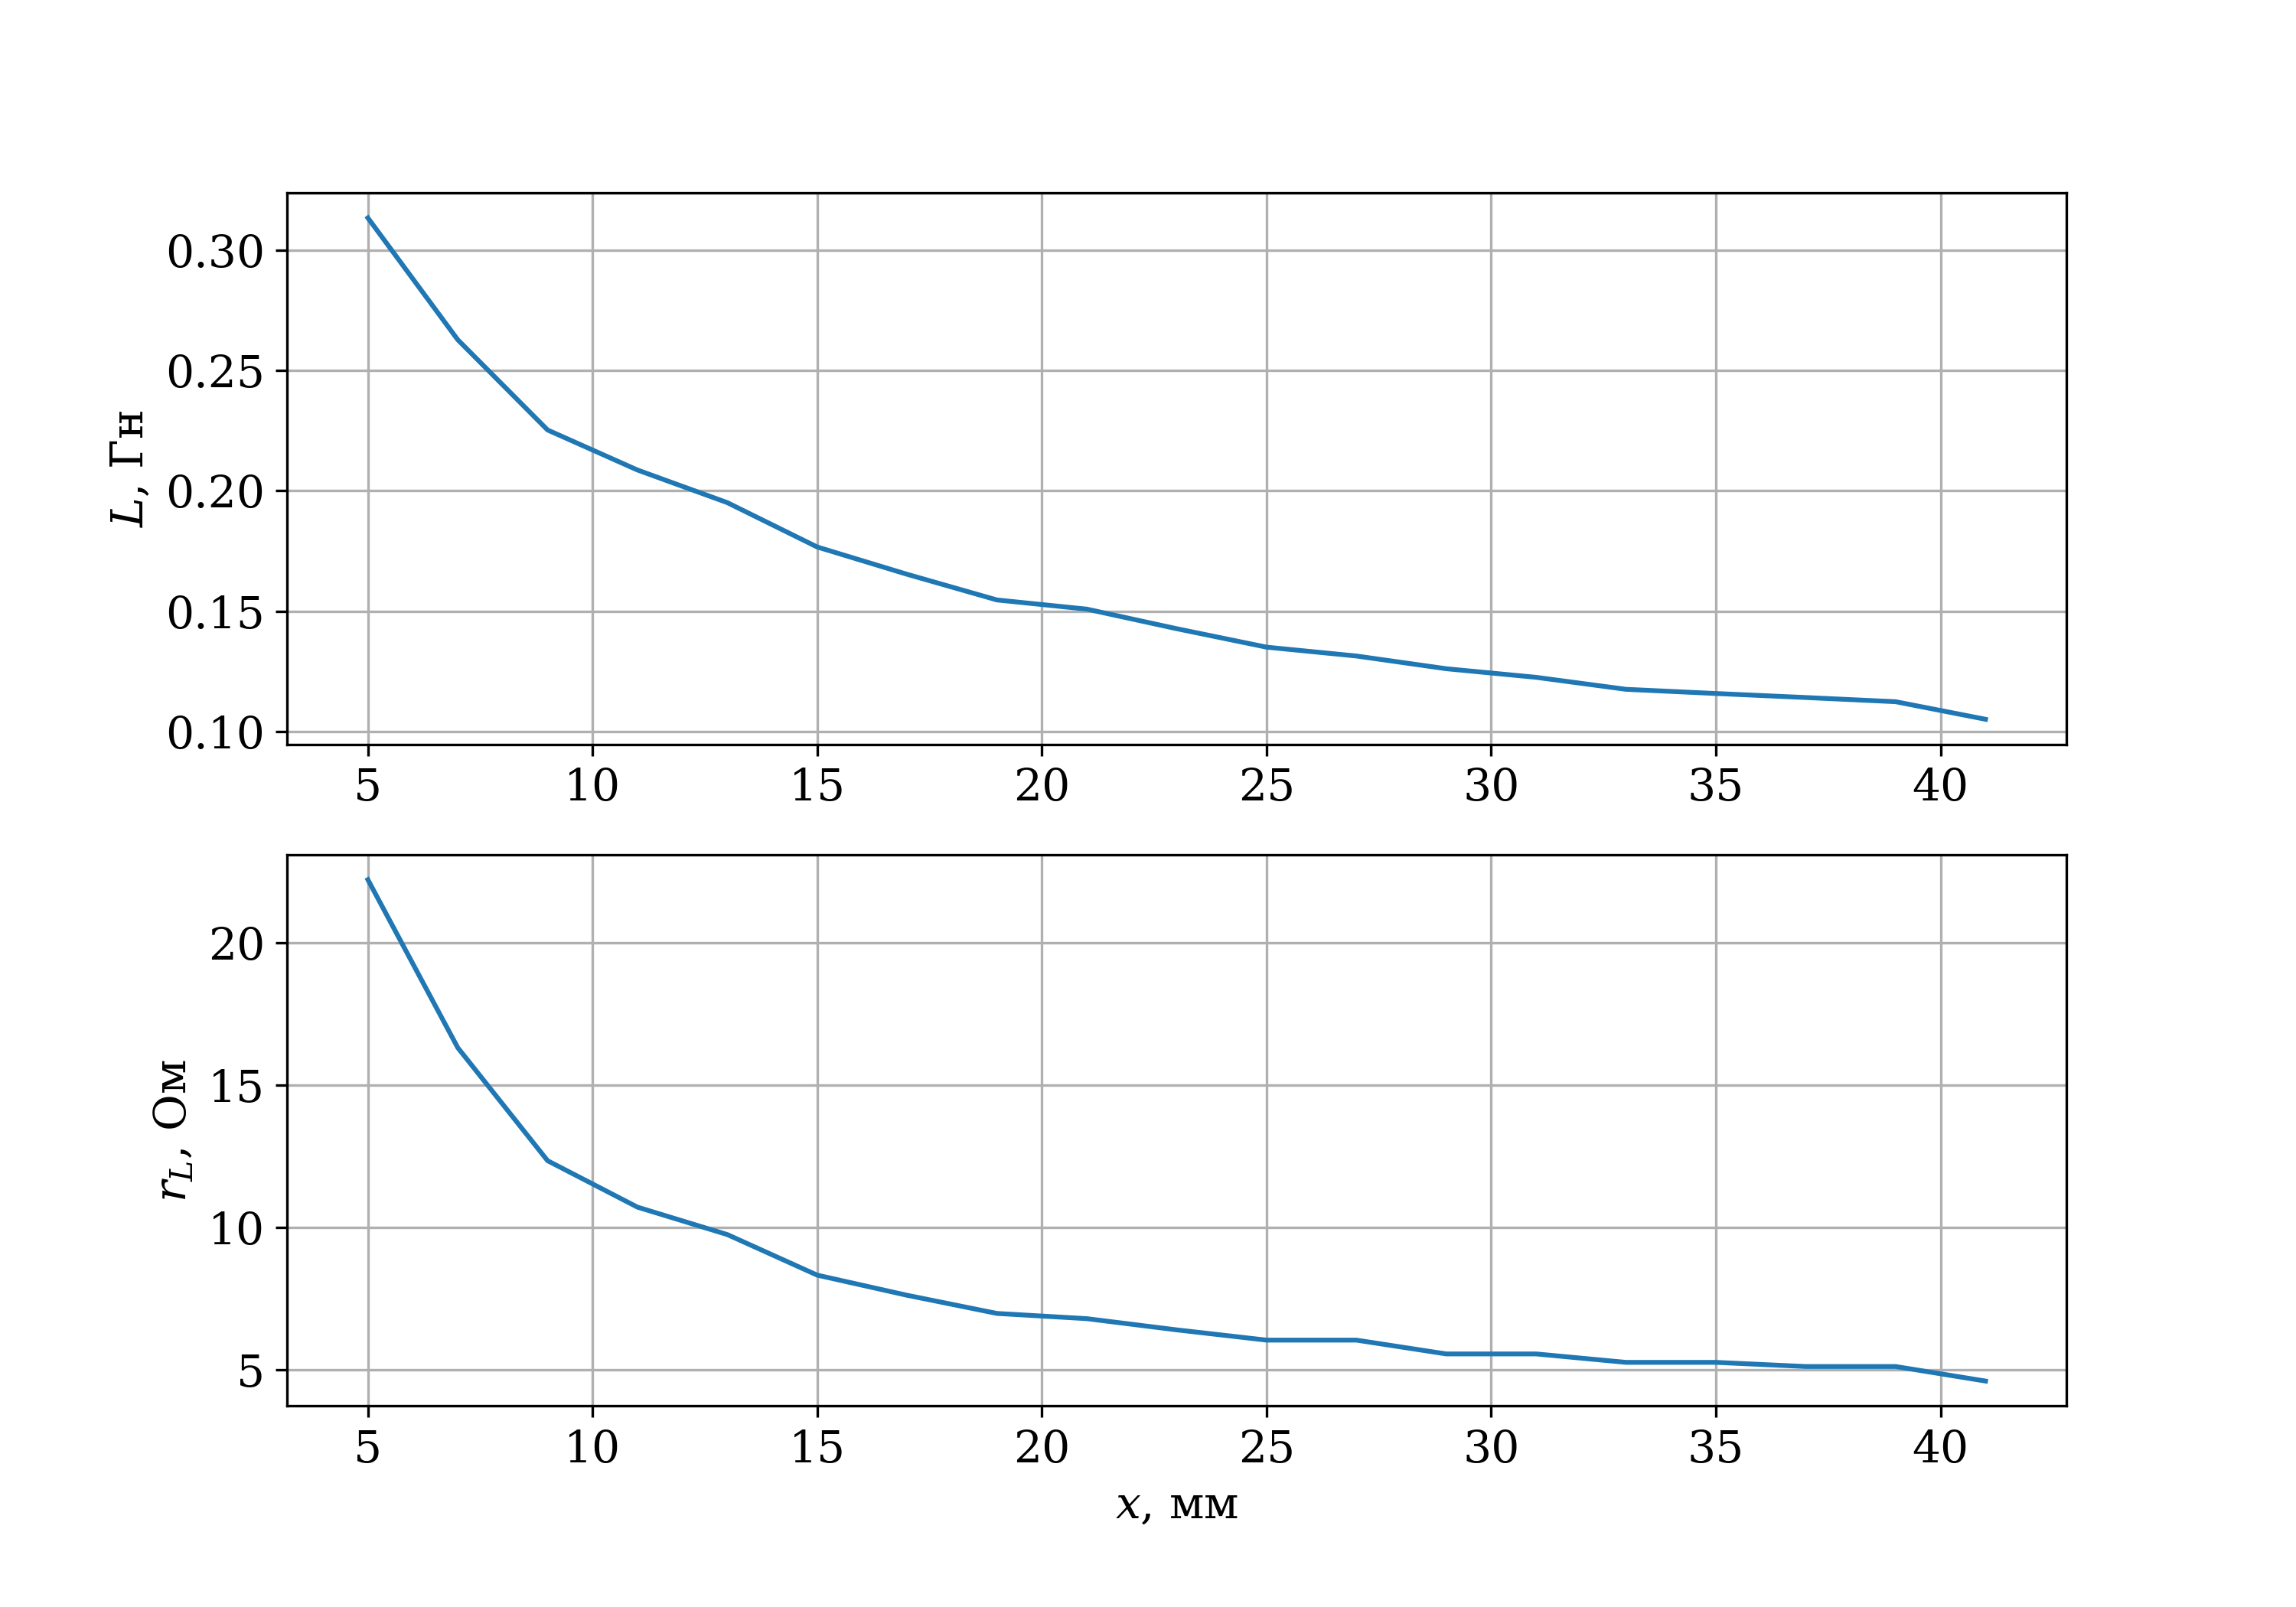
\includegraphics[width=\textwidth]{plot1.png}
\caption{График зависимости индуктивности и активного сопротивления катушки от положения сердечника}
\label{fig:1}
\end{center}
\end{figure}

\paragraph{} Полученные значения индуктивности и активного сопротивления катушки для резонансного положения сердечника: $r_L = 5.1$ Ом, $L = 0.11$ Гн.

\subsection{Исследование векторной диаграммы напряжения}

\paragraph{} Построим векторную диаграмму напряжений $U_L$, $U_R$, $U_{L+R}$ и также компоненты $U_{L, \; \text{реакт}}$ и $U_{L, \; \text{акт}}$ (рис. \ref{fig:2}).

\begin{figure}[h]
\begin{center}
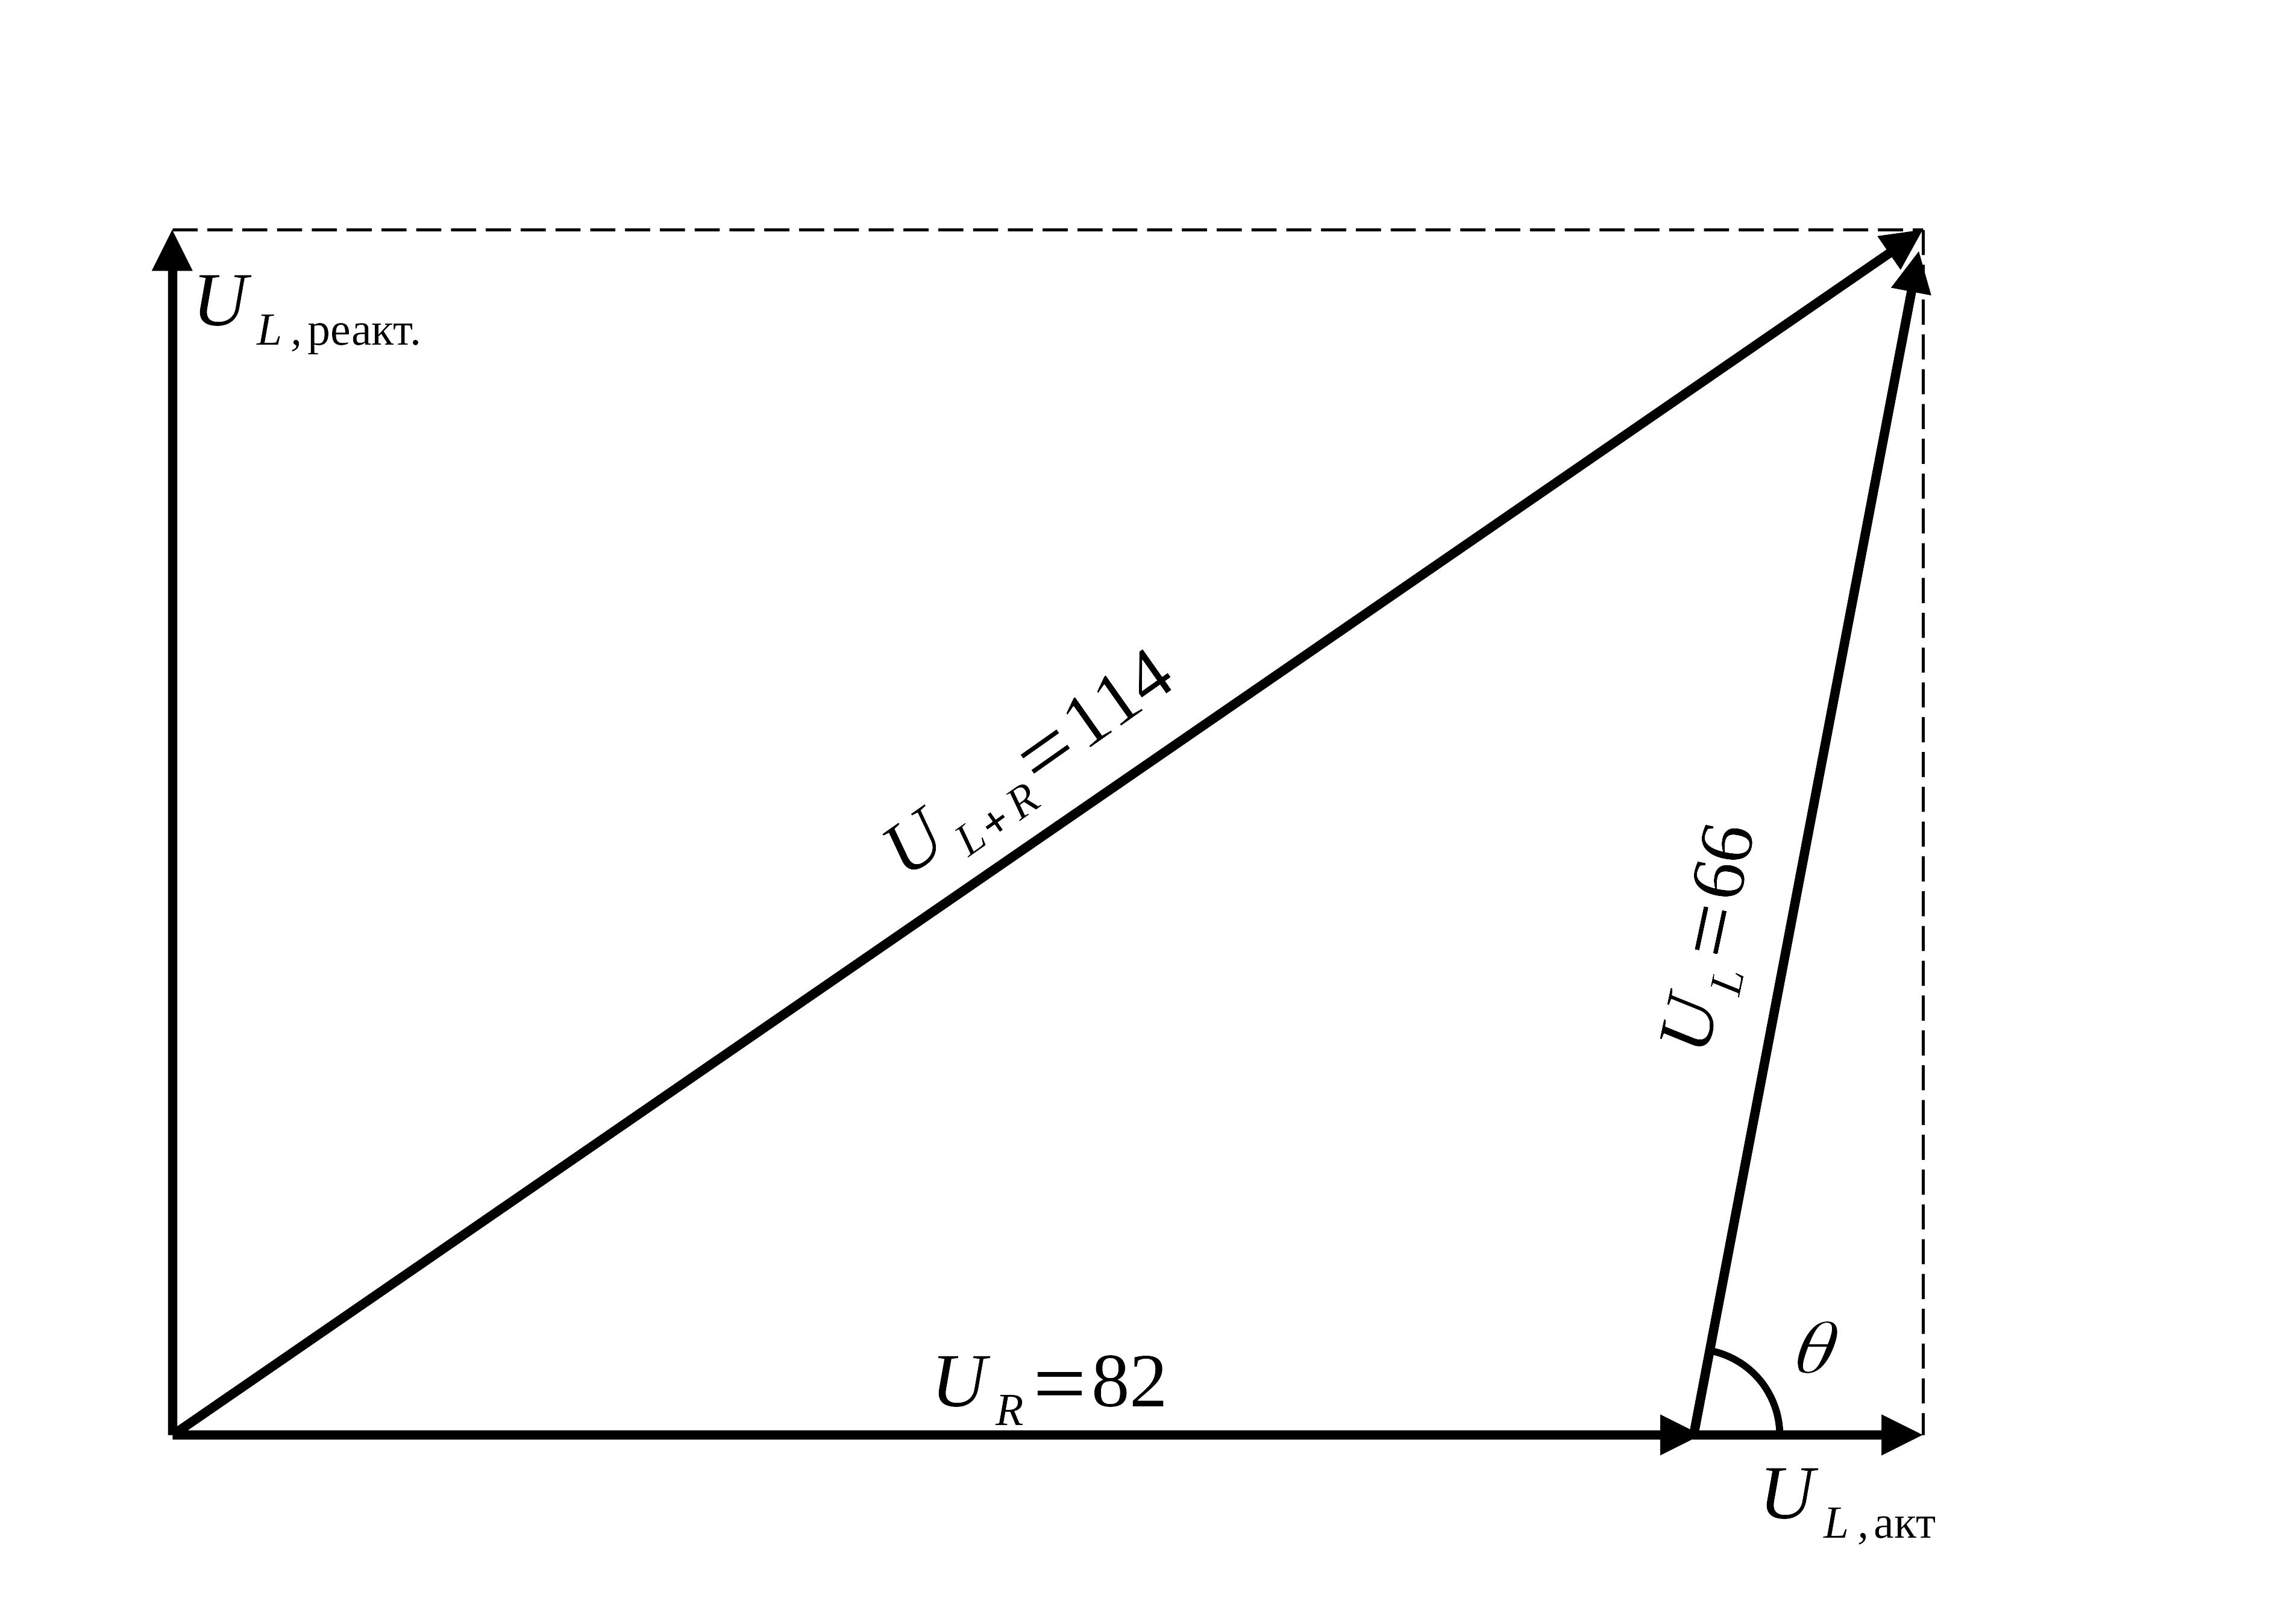
\includegraphics[width=\textwidth]{vector.png}
\caption{Векторная диаграмма}
\label{fig:2}
\end{center}
\end{figure}

\paragraph{} По векторной диаграмме рассчитаем сдвиг фаз между током и напряжением на катушке. По теореме косинусов:

\[ \cos \theta = \frac{U_{L+R}^2 - U_R^2 - U_L^2}{2U_L U_R} = \frac{114^2 - 66^2 - 82^2}{2 * 66 * 82} = 0.178 \; \Rightarrow \; \theta \approx 80 \degree.
\]

\noindent По формуле (\ref{5}) значение $\cos \theta = P_L/(U_L \cdot I) = 0.146 \Rightarrow \theta \approx 81.6 \degree$.

\paragraph{} По векторной диаграмме найдём $r_L$ и $L$:

\[ r_L = \frac{U_{L, \text{акт}}}{I} = \frac{R \cdot U_L}{U_R} \cos \theta = 7.2 \; \text{Ом},
\]

\[ L = \frac{U_{L, \text{реакт}}}{\Omega I} = \frac{R \cdot U_L}{100 \pi \cdot U_R} \sin \theta = 0.12 \; \text{Гн}.
\]

\paragraph{} Также по векторной диаграмме найдём мощность выделяемую на катушке $P_L$, по формуле (\ref{5}):

\[ P_L = U_L \cdot I \cos \theta = \frac{U_L \cdot U_R}{R} = \frac{U_{L+R}^2 - U_R^2 - U_L^2}{2R} = \frac{114^2 - 66^2 - 82^2}{98} = 19.1 \; \text{Вт}.
\] 

\noindent Измеренная при помощи ваттметра мощность $P = 17.5$ Вт.

\medskip\hrule\medskip

\subsection{Исследование резонанса напряжений}

\paragraph{} Соберём установку для исследования резонанса напряжений (рис. \ref{fig:2}). Меняя положение сердечника и ёмкость магазина ёмкости, наблюдая за показаниями ЭО найдём положение резонанса. В этом случае на экране ЭО видна прямая. В положении резонанса ёмкость $C = 44.7$ мкФ, добавочное сопротивление $R_2 = 5.6$ Ом, положение сердечника $x = 39$ мм, напряжения $U_\Sigma = 146$ В, $U_c = 54$ В и ток $I = 2.9$ А.

\paragraph{} Рассчитаем активное сопротивление катушки через ток и напряжение на контуре по формулам (\ref{9}, \ref{7}):

\[ r_L = \frac{U_\Sigma}{I} - 5.6 = \frac{146}{2.9} - 5.6 = 44.7 \; \text{Ом}. 
\] 

\paragraph{} Рассчитаем $L$ и $r_L$ по формуле (\ref{6}, \ref{7}, \ref{10}):

\[ Q = \frac{R_C}{R_\Sigma} = 0.37, \;\;\; r_L = \frac{1}{\omega_0 C Q} - R = 192 \; \text{Ом}.
\]

\[ L = \frac{1}{\omega_0^2 C} = \frac{1}{(100 \pi)^2 \cdot 44.7 \cdot 10^{-6}} = 0.23 \; \text{Гн}.
\]


\section{Выводы}

\paragraph{} Был показан закон Ома для переменного тока на примере векторной диаграммы. И было проведено наблюдение резонанса напряжения на осциллографе. По полученным данными было вычислено несколько величин.

\paragraph{} Полученные данные:

\begin{center}
\begin{tabular}{|c||c|c|c|c|}
\hline 
Способ & I & II & III (1) & III (2) \\ 
\hline 
$r_L$, Ом & 5.1 & 7.2 & 44.7 & 192 \\ 
\hline 
$L$, Гн & 0.11 & 0.12 & -- & 0.23 \\ 
\hline 
\end{tabular} 
\end{center}


\paragraph{} Данные, полученные I и II способами оказались похожими, однако в данных полученных для резонанса данные сильно отличаются. Возможной причиной является неправильно измеренные значения для $C$ и $R_2$.

\medskip\hrule\medskip

\end{document}
